\documentclass[a4paper,10pt]{report}
\usepackage[T1]{fontenc}
\usepackage[table]{xcolor}
\usepackage{titlesec}
\usepackage{graphicx}
\usepackage[inkscapepath=../assets/svg]{svg}
\usepackage{amsmath}
\usepackage{amsthm}
\usepackage{mathtools}
\usepackage{fancyvrb}
\usepackage[english]{babel}
\usepackage{csquotes}
\usepackage{verbatim}
\usepackage{hyperref}
\hypersetup{
   colorlinks=true,
   linkcolor=blue,
   urlcolor=cyan
}
\usepackage{tikz}
\usepackage{amssymb}
\usepackage[sc]{mathpazo}
\linespread{1.05}
\usepackage{microtype}
\usepackage{breqn}
\usepackage{caption}
\usepackage{subcaption}
\usepackage[
   backend=bibtex,%
   bibencoding=utf8,%
   language=english,%
   style=numeric-comp,%
   sorting=nyt,%
   maxbibnames=10,%
   natbib=true%
]{biblatex}
\addbibresource{references.bib}
\usepackage{siunitx}
\usepackage{booktabs}
\usepackage{longtable}
\usepackage{geometry}
\usepackage{multirow}
\graphicspath{ {../assets/img/} }

\newgeometry{hmargin={30mm,30mm}}

% Set TOC depth and sections numbering
\setcounter{tocdepth}{3}
\setcounter{secnumdepth}{3}

% Remove chapters head and reduce spacing
\titleformat{\chapter}[hang]{\Large\bfseries}{\thechapter \hspace{2ex}}{0pt}{\Large}
\titlespacing{\chapter}{0cm}{0cm}{0.5cm}
\usepackage[parfill]{parskip}

% Make quotes italic
\renewcommand{\mkbegdispquote}[2]{\itshape}

% Change texttt line breaks
\renewcommand{\texttt}[1]{%
  \begingroup
  \ttfamily
  \begingroup\lccode`~=`.\lowercase{\endgroup\def~}{.\discretionary{}{}{}}%
  \catcode`/=\active\catcode`[=\active\catcode`.=\active
  \scantokens{#1\noexpand}%
  \endgroup
}


\begin{document}
\frenchspacing

% First page
\title{
  {{\large{\textsc{Alma Mater Studiorum $\cdot$ University of Bologna}}}}
  \rule{\textwidth}{0.4pt}\vspace{3mm}
  \textbf{SKA Data Challenge\footnote{The code for the project is publicly available on \href{https://github.com/Lorenz92/SKADC1}{GitHub}}}
  \begin{figure}[!htb]
    \centering
    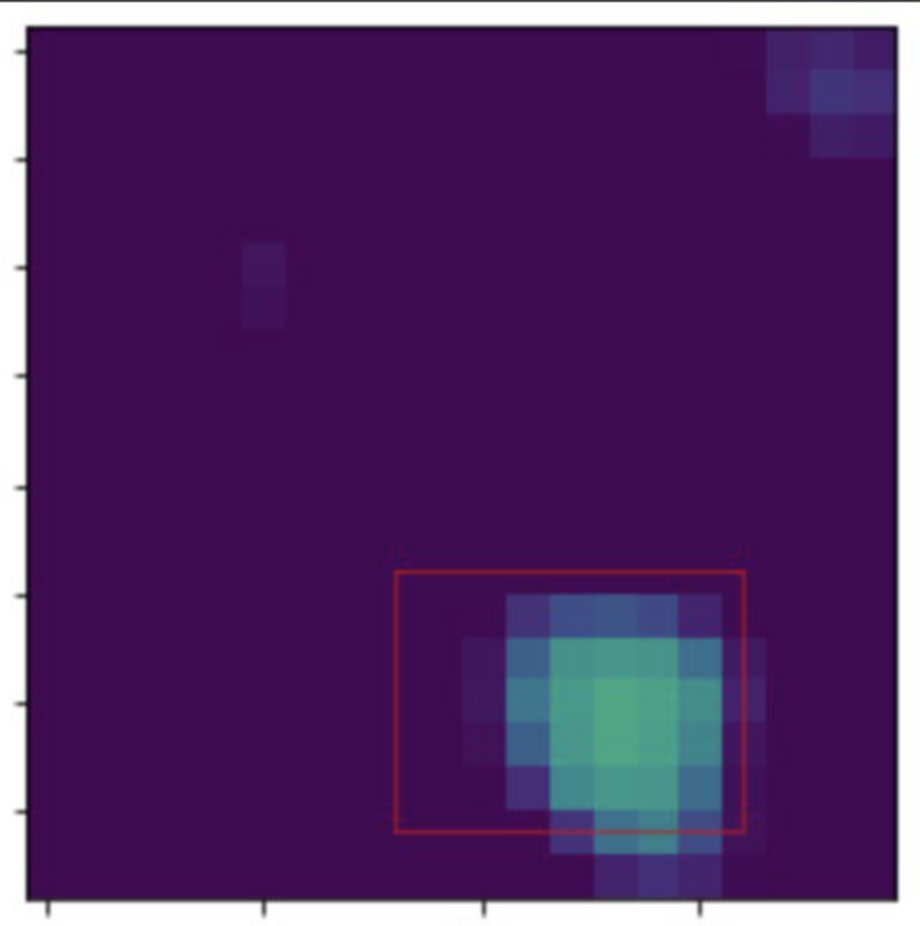
\includegraphics[width = 100pt]{nice-detection.png}
  \end{figure} \\
  Deep Learning course final project
}

\author{Lorenzo Cellini (\href{mailto:lorenzo.cellini3@studio.unibo.it}{lorenzo.cellini3@studio.unibo.it}) \\ Alice Zandegiacomo (\href{mailto:alice.zandegiacomo@studio.unibo.it}{alice.zandegiacomo@studio.unibo.it})}
\date{\today}
\maketitle
\newpage
\tableofcontents
\setcounter{tocdepth}{1}
%\listoffigures
%\listoftables
\newpage


\chapter{Summary}\label{chap:introduction}

The tasks of object detection and classification have gained significant popularity over the past years within the deep learning and computer vision communities. Systems trained end-to-end now achieve great results on a variety of tasks in the video and image domains.

In this work, we address an object detection and classification problem on the Square Kilometer Array Dataset (SKADC1) \cite{ska-site}: given a large image, of about $32000$ pixels on each side and 4GB in size, the goal is to detect astronomycal sources and classify them among three possible classes.

This project focuses on the SKADC1 dataset, in particular on the 560MHz-1000h high S/N sky image, that contains more than \num{19000} radio sources.

Among the state of the art types of network, we opted for a two-stage system, specifically a Faster R-CNN.

In this work we implemented and compared three different models:
\begin{enumerate}
  \item B16: a Faster R-CNN with a naive feature extraction backbone with only 4 convolutional layers and with a receptive field of 16 on the last convolutional layer, that will act as our baseline model;
  \item B44: a Faster R-CNN with a feature extraction backbone with 7 convolutional layers and a receptive field of 44 on the last convolutional layer;
  \item A Faster R-CNN with a larger backbone, specifically we implemented a VGG16 backbone without the last max pooling layer, with a receptive filed of 196 \cite{vgg}.
\end{enumerate}
Each model consists of the same input and output (Region Proposal Network + Detector) structure, and what changes is the deepness of the feature extraction network (usually called backbone).

In training the listed models, we adopted a transfer learning technique, because it has been proven to be effective in speeding up the training phase \cite{claran},\cite{transfer-learning-1}, \cite{transfer-learning-2}.
More specifically, we applied transfer learning only on the very first layers in order to inherit and retain the more basic feature, while letting the model learn deeper representation of them.

While this could seem an easy object detecion and classification problem, it turns out that it is an hard task on both the goals:
\begin{itemize}
  \item the objects to be located are very small, as we will show later, and
  \item the dataset is extremely unbalanced with respect to class distribution.
\end{itemize}

For this two reasons we developed more than one model and we made some choices that will be discussed later.

Our experimental evaluations show that the best model is  ...

\chapter{Background}\label{chap:background}
Our project is an object recognition tasks, which is a general term to describe the identification of objects
in digital photos. 
The object recognition task consists in two aspects: object localization, which implies the drawing of an 
axis-aligned  bounding box around one or more objects, and classification which consists in predicting the class 
of objects.

Among the state of the art top-performing deep learning models for object detection there are:
\begin{itemize}
\item R-CNN (Region-Based Convolutional Neural Network ) Model Family: it was firstly introduced by Girshick et al. in 2014 \cite{rcnn}, then it was improved with the Fast \cite{fast-rcnn} and Faster R-CNN in 2015 \cite{faster-rcnn}, and finally with the Mask R-CNN in 2017 \cite{mask-rcnn}.
In the first version of R-CNN the network involved had the duty to classify and find coordinates of objects on the regions proposed by a Selective Search algorithm that previously ran on the image.The computation of the feature map for each proposed region was carried out separately and this makes the R-CNN very slow. Fast R-CNN improved the execution speed of the first part of the network by computing the feature maps for the whole image and then using the SS proposals to cut feature map regions. The Faster R-CNN \cite{faster-rcnn} substitutes the Selective 
Search of the Fast R-CNN with a Region Proposal Network without loosing accuracy. The Mask R-CNN is similar to the Faster R-CNN, but it uses the feature map to predict not only the class and bounding box for each region of interest, but also the pixel-level position of the object through an additional convolutional network. 
\item YOLO (You Only Look Ones) Model Family: was proposed in 2015 by Joseph Redmon, et al \cite{yolo}. The approach consists in a single neural network trained end to end that takes an image as input and directly predicts bounding boxes and their class labels. The network divides the input image into a SxS grid, where SxS is equal to the width and height of the tensor which presents the final prediction. In case the center of an object is in a grid cell, the gird cell takes responsibility for detecting that object. Moreover, each gird cell is simultaneously responsible for predicting bounding boxes and confidence scores which represent how confident is the model about bounding box containing an object. YOLOv2 uses anchor boxes as Faster R-CNN
\item SSD (Single Shot Detector) was proposed by Wei Liu et al. \cite{ssd} in 2016, with the aim of having the high computational speed of YOLO, while maintaining the accuracy of Faster R-CNN. SSD enhances the speed of running time with respect to Faster R-CNN by eliminating the need of the Region Proposal Network. Therefore, it causes a few drop in mAP, and SSD compensates this by applying some improvements including multiscale features and default boxes. These improvements allow SSD to gain the same of Faster R-CNN using lower resolution images, which then further speeds up the processing of SSD.
\end{itemize}

\chapter{Dataset description}\label{chap:dataset-description}

The data provided by the SKA (Square Kilometer Array) challenge, consists in a series of astronomical high resolution images created through data simulations \cite{bonaldi2021square}.  Images are a simulated SKA continuum image in total intensity at 3 frequencies: 560 MHz, 1.4 GHz and  9.2 GHz, each of witch has 3 different exposures: 8 h, 100 h, 1000 h. For each frequency band a catalogue revealing only a fraction of the simulated galaxies was released. We choose to analyse the image at 560 MHz with 1000 hours of exposure. 

\section{Ground truth data} \label{sec:ground_truth_data}
Each row of the ground-truth catalogue contains the subsequent information of the correspondent source: 
\begin{itemize}
    \item RA (core)  [degs]    Right ascension of the source core
    \item DEC (core)    [degs]    Declination of the source core
    \item RA (centroid)    [degs]    Right ascension of the source centroid
    \item DEC (centroid)    [degs]    Declination of the source centroid
    \item FLUX    [Jy]    integrated flux density
    \item Core frac    [none]    integrated flux density of core/total
    \item  BMAJ    [arcsec]    major axis dimension
    \item  BMIN    [arcsec]    minor axis dimension
    \item  PA    [degs] PA (measured clockwise from the longitude-wise direction)
    \item    SIZE    [none]    1,2,3 for LAS, Gaussian, Exponential
    \item    CLASS    [none]    1,2,3 for SS-AGNs, FS-AGNs,SFGs
    \item  SELECTION    [none]  0,1 to record that the source has not/has been injected in the simulated map due to noise level
    \item    x    [none]    pixel x coordinate of the centroid, starting from 0
    \item   y    [none]    pixel y coordinate of the centroid,starting from 0
\end{itemize}
We used declination, right ascension, minor and major axis to obtain the pixel coordinates of the source center and its bounding box. At first we tried to filter the dataset out using the flux information and the primary beam given by the SKA challenge in order to discard sources with too low signal to noise ratio, but, at the end, we decided to adopt the cleaned dataset courtesy of the ICRAR group (The International Centre for Radio Astronomy Research ) to have a comparison with their results.

We discarded all sources with SELECTION equal to 0 and assigned to each source a class label, given by the concatenation of SIZE and CLASS. In total there are 5 classes. 

An analysis of the distribution of the classes shows that the dataset is highly unbalanced, as can be seen from the scatter plots in table \ref{table:class_analysis}. In particular class $2\_3$ is highly represented, while the number of sources for the other classes is 2-3 orders of magnitude lower. We also analyzed the distribution of height and width by classes: the dimensions seem to be isotropic, but the standard deviation is very high for some classes, while extremely low for others. This can be seen in the scatter plot in \ref{fig:scatter_class}.
Balancing this dataset is a tricky task because patches contain several sources of different classes, depending on patch dimension. Indeed we tried two different approach to overcome this problem: find and re-sample patches that contain only the rare classes and use focal loss for the classification task.
\begin{table}[h]
  \center
  \begin{tabular}{|c|c|c|c|c|}
    \hline
    \textbf{CLASS}& \textbf{number of sources} & \textbf{width (px)} & \textbf{height (px)} \\ 
    \hline
    \textbf{1_1} & 112 & $15.9\pm21.9$ & $15.1\pm13.2$ \\ 
    \hline
    \textbf{2_1} & 34 & $6.2\pm1.3$ & $6.2\pm1.5$ \\ 
    \hline
    \textbf{2_2} & 262 & $5.0\pm0.2$ & $5.0\pm0.2$ \\ 
    \hline
    \textbf{3_3} & 234 & $16.1\pm8.1$ & $17.6\pm10.8$ \\ 
    \hline
    \textbf{2_3} & 18580 & $6.0\pm2.1$ & $6.1\pm2.0$ \\ 
    \hline
  \end{tabular}
  \caption{Number of sources, width and height distribution for each class}
  \label{table:class_analysis}
\end{table}

\begin{figure}[h]
  \center
  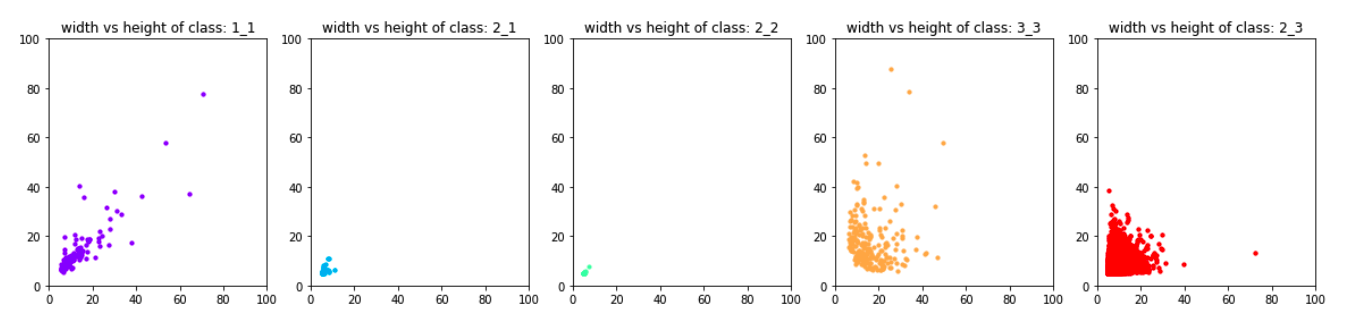
\includegraphics[width=0.85\linewidth]{scatter_class.png}
  \caption{Dataset class distribution}
  \label{fig:scatter_class}
\end{figure}

\section{Image analysis and preprocessing}
The image size is 32768x32768 pixels while the portion of the image that contains the ground truth boxes is around 4000x4000 pixels.
Images were given in FITS format. Since they are a simulation of a radiotelescope acquisition the range of each pixel should be between 0 and 1.
The brightest source in the fits image has value of 0.006586 while the minimum gray level is  $-1.9 \times 10^{-6}$ due to noise simulation.

We converted the pixel value range from [0,1] to [0,255] experimenting with different approaches: firstly we applied a linear transformation considering the maximum GL value as 255 and set the lower value equal to 0. In this way we removed the negative noise signal. Unfortunately, because the sources intensity was not linearly distributed in the range [0,1], but the majority of them had a very low intensity, the resulting image was almost completely black with the exception of very few sources and most of the ground truth boxes were undetectable, \ref{fig:image_transf} (on the left).

The second attempt was using a $\gamma$ function in order to enhance the signal of low intensity sources. We tried several $\gamma$ values between 0.2 and 1, but again many sources were too dark.

Finally, the chosen method was to scale the image intensity range using a base 10 logarithm scale: the magnitude range was defined by the magnitude of the noise standard deviation and of the maximum gray value, \ref{fig:image_transf} (on the rigth). Indeed, the image noise is caused by electronic noise and is well fitted by a Gaussian distribution centered in zero. We obtained the standard deviation looking at the negative values of the gray level distribution, which are necessary caused by noise, and we use it to scale pixel values up.

\begin{figure}[!htb]
  \minipage{0.5\textwidth}
    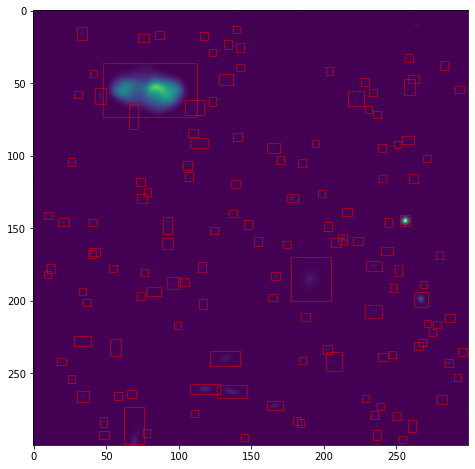
\includegraphics[width=\linewidth]{RGB_linear.png}
  \endminipage\hfill
  \minipage{0.5\textwidth}
    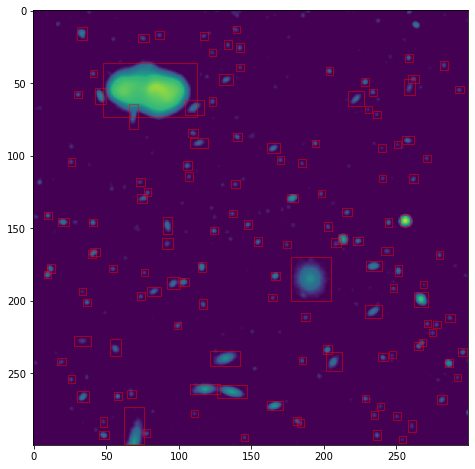
\includegraphics[width=\linewidth]{RGB_log.png}
  \endminipage\hfill
  \caption{Linear transformation on the left and logarithmic transformation on the rigth, of the given image.}
  \label{fig:image_transf}
\end{figure}


\chapter{System description}\label{chap:system-description}

In this work, we implemented three different models. All of them are a Faster R-CNN network and they differ on the backbone and hyperparameters.

In order to perform an effective comparison, the models share the same output architecture.

The following is a detailed description of the models. Beware that in each model section we report everything but what happens in the output layers, which is described once in \ref{sec:output-architecture}.

\section{Feature Extraction Backbone}\label{sec:feature-extraction-backbone}
Basically, in this work we tested:
\begin{enumerate}
\item wether a simple model, meaning "not very deep", is enough for the small and simple-shape object detection task, and;
\item how detection performance varies when changing the receptive field size of the model with respect to objects size.
\end{enumerate}

For this reasons we implemented three different feature extraction backbone with different receptive field size.

\subsection{B16 - Baseline 16}\label{subsec:b16}

The first backbone we implemented has the following structure:
\begin{enumerate}
  \item Block 1: consists of 2 convolutional layers with 3x3x64 filters, followed by a ReLU activation layer and a 2x2 MaxPooling layer with stride 2;
  \item Block 2: consists of 2 convolutional layers with 3x3x128 filters, followed by a ReLU activation layer and a 2x2 MaxPooling layer with stride 2;
\end{enumerate}
Both the blocks have been initialized with the public available VGG16 weights and \textbf{freezed}.

It has been shown that, in computer vision tasks, the very first layers of a convolutional pipeline, learn the most basic features, as strokes or circles \cite{cnn-features}.
So, given that the objects we have to detect have simple shapes, like circles or ellipses, and that we think these kind of basic feature are common across different domains, 
we tried to transfer learning from the VGG16 and freezing the first layers, the ones that learn most basic features.

With the B16 model, we wanted to test how a shallow feature extraction network performs in predicting small and simple shapes objects.

Furthermore, we tested how the relation between the receptive field size and the object size, influences the learning: indeed, B16 has a receptive field size of 16 and this is smaller than any object size for the 20\_100 set, but bigger than the 80\% of the objects in the 50\_100 set. More details in chapter \ref{chap:experiments}.

With this architecture, the final feature map size $r$ is $\frac{1}{4}$ of the input image.

\subsection{B44 - Baseline 44}\label{subsec:b44}
The second backbone we implemented has the following structure:
\begin{enumerate}
  \item Block 1: consists of 2 convolutional layers with 3x3x64 filters, followed by a ReLU activation layer and a 2x2 MaxPooling layer with stride 2;
  \item Block 2: consists of 2 convolutional layers with 3x3x128 filters, followed by a ReLU activation layer and a 2x2 MaxPooling layer with stride 2;
  \item Block 3: consists of 3 convolutional layers with 3x3x256 filters, followed by a ReLU activation layer and a 2x2 MaxPooling layer with stride 2;
\end{enumerate}
The first two blocks are the same as in the B16 model. 

By adding the third block we wanted to test how performance changes with a deeper model.

The purpose of this backbone is also to make a direct performance comparison between B16 and B44 on the same input image size. Indeed, B44 has a receptive field size of 44, that is greater than the 90\% of objects to detect (in the 20\_100 set).

Each block is initialized with the VGG16 weights. Block 1 and 2 have been freezed, while block 3 is left free to learn.

With this architecture, the final feature map size is $\frac{1}{8}$ of the input image.

\subsection{VGG16}\label{subsec:vgg16}
The third backbone we implemented is the well known VGG16 backbone, without the fully connected part and without the last MaxPooling layer.

It has the following structure:
\begin{enumerate}
  \item Block 1: consists of 2 convolutional layers with 3x3x64 filters, followed by a ReLU activation layer and a 2x2 MaxPooling layer with stride 2;
  \item Block 2: consists of 2 convolutional layers with 3x3x128 filters, followed by a ReLU activation layer and a 2x2 MaxPooling layer with stride 2;
  \item Block 3: consists of 3 convolutional layers with 3x3x256 filters, followed by a ReLU activation layer and a 2x2 MaxPooling layer with stride 2;
  \item Block 4: consists of 3 convolutional layers with 3x3x512 filters, followed by a ReLU activation layer and a 2x2 MaxPooling layer with stride 2;
  \item Block 5: consists of 3 convolutional layers with 3x3x512 filters, followed by a ReLU activation layer;
\end{enumerate}
The first two blocks are the same as in the B16 model, while the third is the same as in the B44.

Each block is initialized with the VGG16 weights. Block 1 and 2 have been freezed, while block 3, 4 and 5 are left free to learn. The receptive field of this backbone is 196.

With this architecture, the final feature map size is $\frac{1}{16}$ of the input image.

\section{Output Architecture}\label{sec:output-architecture}
The output architecture is the same as of a standard Faster R-CNN module and consists of a Region Proposal Network (RPN) and a Roi Pooling Layer coupled with a fully connected network that we called "Detector".

This kind of network is called "two-stage" network because the training phase is carried on in two step:
\begin{enumerate}
    \item The feature maps generated by the backbone are feed into the RPN network. It generates a batch of proposals and pass them down to the Detector;
    \item the Detector takes the feature maps and the proposals, uses the latter to cut the corresponding regions on the feature maps and classifies the cuts.
\end{enumerate}
RPN and Detector share the same backbone weights and have distinct loss functions.

Depending on how the network works, the training phase is carried out in a stochastic gradient descent fashion: the network is feed with one single image at a time, but besides the feature extraction backbone there are some specific functions that generate the actual ground truth batch that RPN uses in order to compute its loss. The output of the RPN is then filtered through a non-maximum-suppression algorithm (NMS \cite{nms}) based on the intersection-over-union score (IoU \cite{iou}). From the result, an equal number of positive (foreground) and negative (background) samples are drawn and passed to the Detector. This number is one of the hyper-parameters of the model.

\subsection{Region Proposal Network}\label{subsec:rpn-net}
"A Region Proposal Network (RPN) takes an image (of any size) as input and outputs a set of rectangular object proposals, each with an objectness score." \cite{faster-rcnn}
The structure of this network is the following:
\begin{itemize}
    \item 1 convolutional layer with 3x3x512 filters, initialized with a Gaussian distribution centered in 0 with a stdev of 0.01  \cite{faster-rcnn}, followed by a ReLU activation layer;
    \item 1 convolutional layer with 1x1xnum\_classes filters, initialized with a uniform distribution;
    \item 1 convolutional layer with 1x1x4xnum\_classes filters, initialized to the constant 0.
\end{itemize}

The second layer is in charge to determine the "objectness" score of a candidate region, (which can be interpreted as the probability that the region contains an object) while its sibling, the third layer, is in charge of outputting the difference in coordinates of such proposals with respect to model anchors.

The output of the RPN net goes trough the NMS algorithm based on IoU score. The results is the set of ROI proposals that the Detector will have to classify and locate.

Hyper-parameters of RPN module are:
\begin{itemize}
    \item the number of regions to evaluate: 256;
    \item number of output ROI from NMS: 2000;
    \item NMS positive overlap threshold: 0.7, negative overlap threshold: 0.3.
\end{itemize}

The RPN loss function is:
\[L({p_i}, {t_i}) = \dfrac{1}{N_{cls}^{rpn}} \sum_{i} L_{cls}^{rpn}(p_i, p_i^*) + \lambda \dfrac{1}{N_{reg}^{rpn}} \sum_{i} p_i^* L_{reg}^{rpn}(t_i, t_i^*) \]	
where the first term is the binary cross entropy and represents the loss related to the "objectness" score; the second term is the smooth $L_1$ score as in \cite{huber-loss}. The $p_i^*$ multiplier acts as a kind of mask, activating the regression loss only for positive proposals.

\subsection{Roi Pooling Layer}\label{subsec:roi-pooling}
ROI max pooling works by dividing the $h \times w$ RoI window into an $H \times W$ grid of approximately size $\frac{h}{H} \times \frac{w}{W}$ and then max-pooling the values in each sub-window. Pooling is applied independently to each feature map channel.

ROI pooling layer is needed because the last Faster R-CNN module is a fully connected network that needs fixed-length feature vector as input, but proposals from RPN can have different height and width. So, ROI pooling layer scales down and resizes proposals to a $n \times m$ map, where $n$ and $m$ are model hyper-parameters. We chose $n=m=7$ as in \cite{faster-rcnn}.
\begin{figure}[h]
  \center
  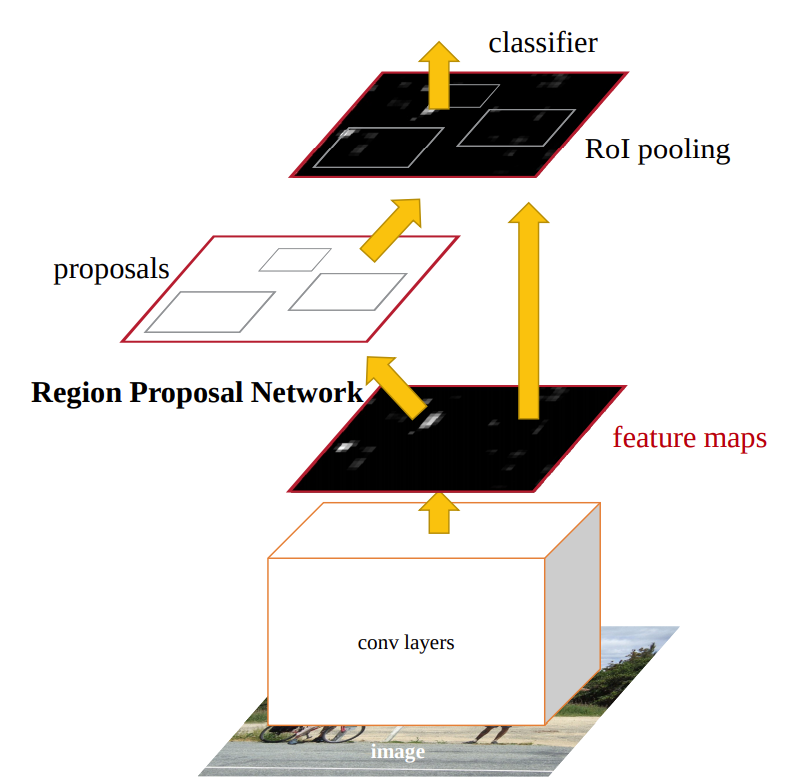
\includegraphics[width=0.5\linewidth]{roi-pooling}
  \caption{ROI Pooling Layer (image courtesy of \cite{roi-pooling})}
  \label{fig:roi-pooling}
\end{figure}

\subsection{Detector}\label{subsec:detector}
The last Faster R-CNN module is a fully connected network that aims to classify RPN proposals among possible object categories and output bounding boxes coordinates refinements.

It consists of:
\begin{itemize}
    \item ROI pooling layer (described above);
    \item 2 fully connected layers with 4096 units and $0.5$ of dropout probability, each one followed by ReLU activation;
    \item 1 fully connected layer with $num\_classes$ units, initialized to 0 and followed by a softmax activation;
    \item 1 fully connected layer with $4*num\_classes$ units, initialized to 0 and followed by a linear activation.
\end{itemize}
In our dataset we had $num\_classes=6$, where 5 were actual classes and the last was the background class.

The model loss is:
\[L({p_i}, {t_i}) = \dfrac{1}{N_{cls}^{det}} \sum_{i} L_{cls}^{det}(q_i, q_i^*) + \lambda \dfrac{1}{N_{reg}^{det}} \sum_{i}L_{reg}^{det}(s_i, s_i^*) \]

where the first term is the categorical cross entropy and represents the classification loss with respect to object classes and the second term is again the $smooth-L_1$ that represents the shift regression from the proposed regions to the actual coordinates shifts.

\subsection{Focal Loss}\label{subsec:focal-loss}
In some of our experiments we also tried to overcome the unbalancedness of the dataset by exploiting focal loss \cite{focal-loss}.
Authors in \cite{focal-loss} proposed focal loss as a way to down weight background examples with respect to foreground ones. Thus they claim that thanks to focal loss it is not necessary to restrict RPN proposal to a fixed number and ratio and to perform biased sampling on the Detector stage.

Anyway we implemented focal loss with a slightly different goal: to help the model to distinguish between rare and common classes positive samples. Indeed we maintained the fixed RPN proposals and applied 1:1 biased sampling to the proposed ROI. In this way we think the model could converge faster, and, once it starts detecting objects, the focal loss should help him better discriminate between classes.
Moreover, in \cite{focal-loss} they proposed focal loss for one-stage detectors, while we applied it to a two-stage detector.

In the experiments where focal loss is applied, the Detector loss becomes:
\[L({p_i}, {t_i}) = \dfrac{1}{N_{cls}^{det}} \sum_{i} FL_{cls}^{det}(q_i, q_i^*) + \lambda \dfrac{1}{N_{reg}^{det}} \sum_{i}L_{reg}^{det}(s_i, s_i^*) \]
where
\[FL_{cls}^{det}(q_i, q_i^*) = \alpha (1-\gamma)^2 CE(q_i, q_i^*)\]
where $CE(q_i, q_i^*)$ is the categorical cross entropy. 

We adopted $\alpha=0.25$ and $\gamma=2$ as the best performing ones found in \cite{focal-loss}.

\chapter{Experimental setup and results}\label{chap:experiments}
 We defined 9 experiments, which are a combination of the three different backbone models discussed before and the following parameters:

\begin{itemize}
    \item dimensions of the input patches: we tried $20 \times 20$, $50 \times 50$ and $100 \times 100$ pixel patches (see section \ref{sec:data-handling}). The patches size causes both a variation in the number of ground truth boxes per patch and their size. The latter because, before feeding the network, we scaled patches up to the network input size: 100x100px for B16 and B44, 600x600px for VGG16.
    \item size and aspect ratio of anchors: for each model we defined a set of anchors given by the combination of their possible sizes and ratios. Anchors are drawn on the input image and the distance between the centers of two anchors sets is given by the stride of the network, being the latter the re-sizing factor between the input image and the last feature map. In this work strides were: 4 for B16, 8 for B44 and 16 for VGG16. Thus, for each model, the number of anchors is $anchor\_sizes \times anchor\_ratios \times feature\_map\_size$, where $feature\_map\_size$ is in the $r \times r$ format.
    \item focal loss and dataset balancing: as shown in section \ref{sec:ground_truth_data} the dataset is strongly unbalanced, so we tried to overcome this by using focal loss (cap \ref{subsec:focal-loss}) or by balancing the training dataset (section \ref{sec:data-handling}). These two approaches have been applied separately in different training configurations in order to make a meaningful comparison.  
    \item normalization of the values of the input patches: in some of the experiments, patches pixel values have been normalized by dividing for the max patch pixel value. A more detailed explanation is given in the next section.
\end{itemize}

In table \ref{table:experimental_setup} and following chapters we adopt the nomenclature \emph{baseline\_n\_m + FL(focal loss) or BD (balanced dataset)} to unequivocally identify the combination of feature extraction backbone and parameters used in the various tests. Here $n$ and $m$ represent the original patches dimension and the dimension after patch resizing.

\begin{table}[t]
    \center
    
\resizebox{\textwidth}{!}{%
    \begin{tabular}{|l|c|c|c|c|c|c|c|}
      \hline
      \textbf{Test name}&  \textbf{Rec. field}& \textbf{Patch(px)}& \textbf{Input(px)} & \textbf{Anchors} & \textbf{Norm.} & \textbf{Focal loss} & \textbf{Balancing} \\ 
      \hline
      \textbf{B16_50_100} & 16 &50x50 &100x100  & \shortstack{[8,16,32,64] \\ {[1:1,1:2,2:1]}} & Yes  & No & No \\
      \hline
      \textbf{B16_50_100+FL} & 16 &50x50 &100x100  & \shortstack{[4,8,16,32,64] \\ {[1:1,1:2,2:1]}} & Yes  & Yes & No \\
      \hline
      \textbf{B16_50_100+BD} & 16 &50x50 &100x100  & \shortstack{[8,16,32,64] \\ {[1:1,1:2,2:1]}} & Yes  & No & Yes \\
      \hline
      \textbf{B16_20_100} & 16 &20x20 &100x100 & \shortstack{[4,8,16,24,32,64] \\ {[1:1,1:2,2:1]}} & Yes  & No & No \\
      \hline
      \textbf{B16_20_100+FL} & 16 &20x20 &100x100 & \shortstack{[4,8,16,24,32,64] \\ {[1:1,1:2,2:1]}} & Yes  & Yes & No \\
      \hline
      \textbf{B16_20_100+BD} & 16 &20x20 &100x100 & \shortstack{[4,8,16,24,32,64] \\ {[1:1,1:2,2:1]}} & Yes  & No & Yes \\
      \hline
      \textbf{B44_  } & 44  &20x20 &100x100  & \shortstack{[4,8,16,24,32,64] \\ {[1:1,1:2,2:1]}}  & - & - & - \\
      \hline
      \textbf{VGG16_100_600} & 196 & 100x100 &600x600 & \shortstack{[32,64,128] \\ {[1:1,1:2,2:1]}} & No  & No & No \\
      \hline
    \end{tabular}}
    \caption{Experiments setup, defined by: test name, receptive field of the feature extraction backbone, patch size, anchors size and ratio, normalization of the gray level values, whether focal loss or balancing were used.}
    \label{table:experimental_setup}
  \end{table}
 
The hyperparameters listed in table \ref{table:hyperparameters} were mainly taken from \cite{faster-rcnn}, in order to have a well-established benchmark, even though some of them were adjusted based on available resources (e.g. epochs num) or on our personal thoughts (e.g. we think that increasing Detector ROI would speed the training up).

In each test, 1 epoch consisted in 250 iterations.

\section{Receptive Field}\label{sec:receptive-field}
\begin{figure}[h]
  \center
  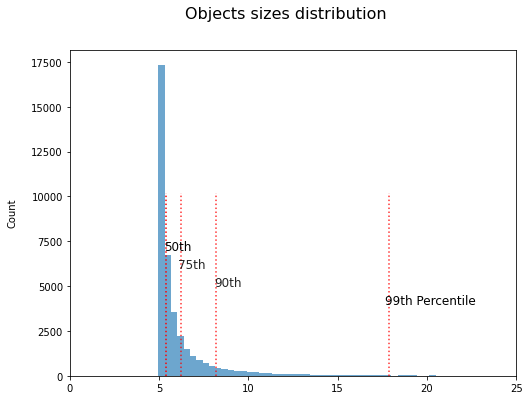
\includegraphics[width=0.65\linewidth]{objects_dist.png}
  \caption{Objects size distribution.}
  \label{fig:objects_dist}
\end{figure}
In this section we want to remark one of the central aspects of this project: we experimented on how the network receptive field interacts with the size of objects to be detected. Indeed we developed 3 different feature extraction backbones with different receptive field size.

As depicted in \ref{fig:objects_dist}, the ground truth shapes distribution shows that the 99\% of the objects is smaller than $18 \times 18$ pixels and the 90\% is smaller then $8 \times 8$ pixels, before patch resizing.

In the \emph{20\_100} set, after resizing the distribution becomes: 99\% smaller than $90 \times 90$ pixels and 90\% smaller then $40 \time 40$ pixels.
We used this set to feed B16 and B44 models that have respectively a receptive field size smaller then the 100\% of objects to detect (B16) and bigger then the 90\% of objects (B44).

In the \emph{50\_100} set, after resizing the distribution becomes: 99\% smaller than 36x36 pixels and 90\% smaller then 16x16 pixels.
We used this set with B16 that has a receptive field equal to the size of 90\% of objects to detect.

In the \emph{100\_600} set, after resizing the distribution becomes: 99\% smaller than 108x108 pixels and 90\% smaller then 48x48 pixels.
We used this set with VGG16, which has a receptive field size of 196, bigger then any object to be detected.

We will discuss in \ref{chap:discussion} how the receptive field influenced the results.
\begin{table}[t]
    \center
    \resizebox{\textwidth}{!}{%
    \begin{tabular}{|c|c|c|c|c|c|c|}
      \hline
                          & \textbf{Epochs} & \textbf{RPN regions} & \textbf{Detector ROI} & \textbf{NMS neg-pos} & \textbf{Optimizer} & \textbf{Learning rate} \\ \hline
      \textbf{B16}   & $200$            & $256$ & $16$ & $0.7-0.3$ & Adam & $1e-2$ \\ \hline
      \textbf{B44}      & $400$            & $256$ & $16$ & $0.7-0.3$ & Adam & $1e-2$ \\ \hline
      \textbf{VGG16}       & $30$            & $256$ & $16$ & $0.7-0.3$ & Adam & $1e-2$ \\ \hline
    \end{tabular}}
    \caption{Hyperparameters}
    \label{table:hyperparameters}
  \end{table}
 
\section{Data pre-processing}\label{sec:data-handling}
Given the image and the dataset described in \ref{chap:dataset-description} we firstly cut out an around $4000$x$4000$px image from the original image: this is the region that contains the ground truths from the dataset.
Then we generated 3 set of patches, $[20\_100]$, $[50\_100]$, $[100\_600]$, in order to run different experiments. In the naming convention $[n\_m]$, $n$ is the size of the cut out patch from the $4000$x$4000$px image, and $m$ is the scaled patch size before feeding the network.

During patches generation we cut a square of side $\sqrt{10000}$ in order to have a maximum amount of $10000$ patches. We decided to use a step of size $\frac{n}{2}$ in order to avoid to lose the complete shape of the objects.
From this set we removed patches with no ground truth, patches that contained part of blacklisted objects and patches smaller then $n$. The latter was in order to avoid issues on borders.
We also discarded objects if they were captured for less than $80\%$ of their surface.

Each patch was casted to the range 0-255 using the base 10 logarithmic scale, where the minimum value is given by the standard deviation of the noise computed over the entire image, while the maximum value is given by the magnitude of the highest value in the patch. 

At training time we normalized patches values by dividing for their maximum value. We also tried zero-centering as in \cite{claran} but we discovered that patch normalization worked best.

Before feeding the network we replicated the same input image 3 times, one for each channel. Our code supports also an "Expander" layer, a 1x1x3 convolutional layer that converts a 1-channel image into a 3-channel one. At the end we decided to not use this layer based on experimental evidences.

Our code supports also augmentation on the fly, and in particular we implemented horizontal and vertical flipping, and the four 90° rotations. However we think this is not strictly necessary in this specific problem because shapes to be predicted are isomorphic with no intrinsic orientation. So we used it only when we balanced the dataset in order to add some training noise.

Regarding the splitting strategy for the dataset, we went for a simple holdout, thus setting aside $20\%$ of the whole dataset for validation purposes. 
During splitting we can also decide whether to balance the dataset: we ran different experiments in order to compare this strategy with the focal loss mentioned in \ref{subsec:focal-loss}.
In order to balance the dataset we simply find patches that contains the rare classes alone, we compute the frequencies of rare classes and we sample with repetition from these sets until the final class distribution becomes uniform. As it is this approach is not very robust, but it can be made better coupling the balancing with the augmentation described before.

We decided to run all of our experiments on a total amount of 350 patches, where 280 for the training set and 70 for the evaluation set. Obviously objects contained in a patch varies depending on the $n$, the patch size.

Figures \ref{fig:20_100}, \ref{fig:50_100} and \ref{fig:100_600} show the class distribution for the three set of input patches.

\begin{figure}[h]
  \center
  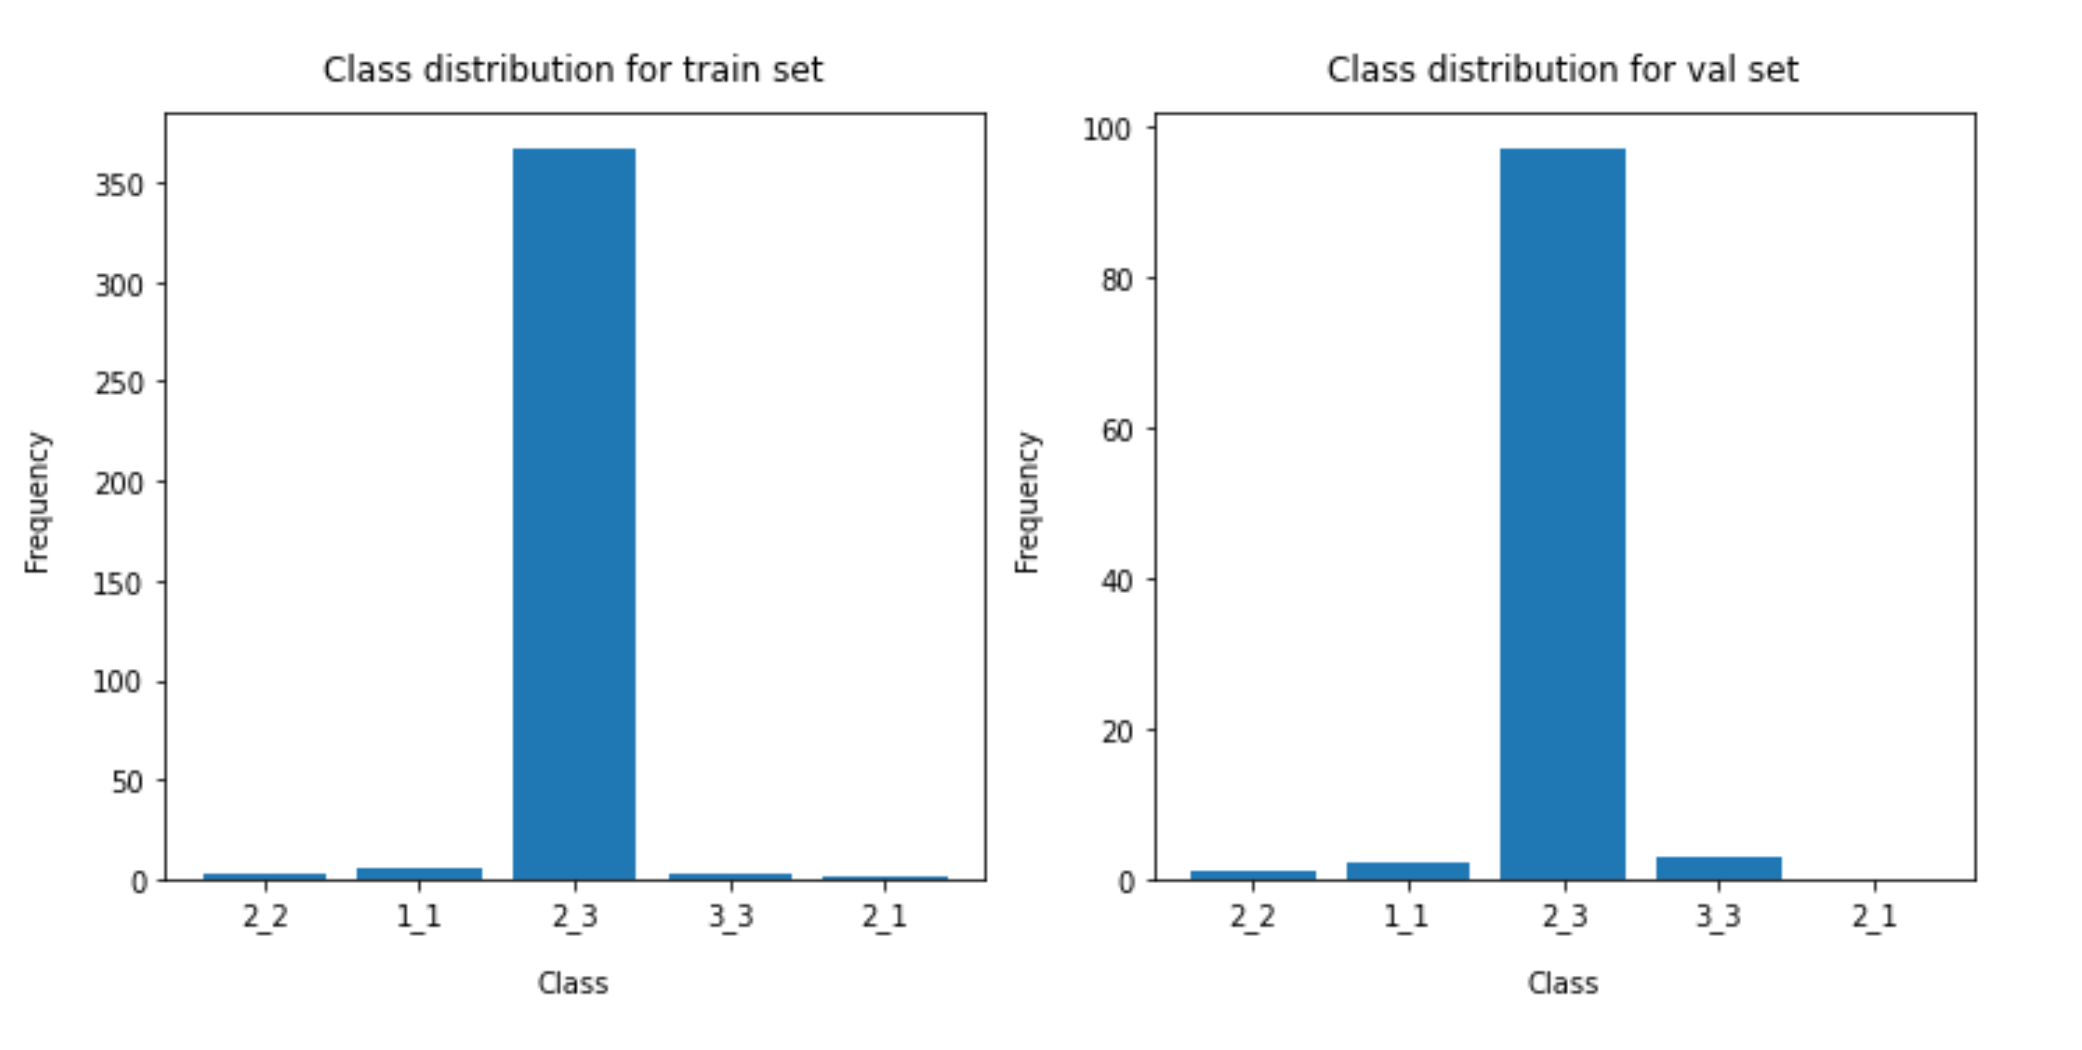
\includegraphics[width=0.65\linewidth]{20_100.png}
  \caption{Class distribution for 20_100 set}
  \label{fig:20_100}
\end{figure}
\begin{figure}[h]
  \center
  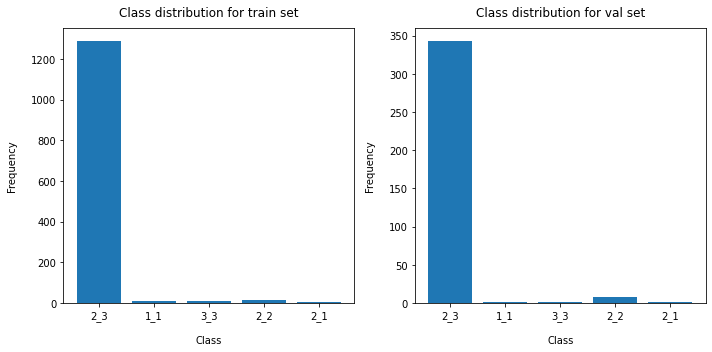
\includegraphics[width=0.65\linewidth]{50_100.png}
  \caption{Class distribution for 50_100 set}
  \label{fig:50_100}
\end{figure}
\begin{figure}[h]
  \center
  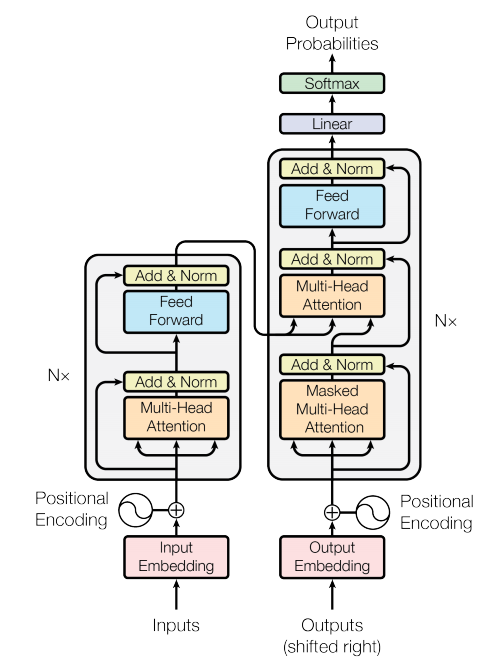
\includegraphics[width=0.65\linewidth]{100_600.png}
  \caption{Class distribution for 100_600 set}
  \label{fig:100_600}
\end{figure}

\section{Metrics}
Metrics adopted to evaluate the models are mAP for the IoU threshold $0.5$, macro-precision and macro-recall.
The evaluation step is carried out at the end of each epoch: in this way we track metrics on validation set and save weights when mAP increases.[citazione per giustificare map]
On the training set we track the four losses and classification accuracy of Detector.

\section{Environment}
The main third-party libraries on which the project is based on are Tensorflow \cite{tensorflow} and Keras \cite{keras}, being the first a machine learning system that operates at large scale and in heterogeneous environments and the latter an API that speeds deep learning model implementation up.

All of the training and validation processes were executed on a MacBook Pro with 2GHz Intel Core i5 quad-core, 16 GB RAM and an Intel Iris Plus Graphics 1536 MB, and on a Dell Precision 5540, 2.60 GHz Intel core i7, 16 Gb RAM.

We tried also to use Google Colaboratory \cite{colab}, a platform that gives the possibility to exploit some computational resources for free, but because of its commercial limits, after few hours of batch computation they cut down our resources and training of models became 30x slower than on the MacBook.

\section{Results}\label{sec:results}
Table \ref{table:results} shows the results obtained on the test set for each model, with the hyperparameters listed in table \ref{table:hyperparameters}.
Unfortunately, VGG16 required a lot of computational resources and we couldn't manage to train it for more than 30 epochs. Anyway, the first 2000 iterations of a Faster R-CNN are usually considered as warm-up \cite{warm-up} and in our case VGG16 ran for a total of 7500 iterations.

\begin{table}[h]
    \center
    \resizebox{\textwidth}{!}{%
    \begin{tabular}{|l|c|c|c|c|c|c|}
      \hline
      \multirow{2}{*}{}   & \multicolumn{3}{c|}{\textbf{Training}} & \multicolumn{3}{c|}{\textbf{Test}}                                                          \\ \cline{2-7}
                          & \textbf{mAP\textsubscript{.5}} (\%) & \textbf{mPrec} (\%) & \textbf{mRec} (\%) & \textbf{mAP\textsubscript{.5}} (\%) & \textbf{mPrec} (\%) & \textbf{mRec} (\%)  \\ \hline
      \textbf{B16_50_100}           & $$ & $$ & $$ & $$ & $$ & $$ \\ \hline
      \textbf{B16_50_100 + FL}      & $41.72$ & $3.13$ & $3.73$ & $\textbf{42.17}$ & $1.77$ & $1.63$ \\ \hline
      \textbf{B16_50_100 + BD}      & $-$ & $-$ & $-$ & $-$ & $-$ & $-$ \\ \hline
      \textbf{B16_20_100}         & $\textbf{41.74}$ & $\textbf{23.29}$ & $\textbf{38.27}$ & $\textbf{39.50}$ & $\textbf{23.64}$ & $\textbf{43.45}$ \\ \hline
      \textbf{B16_20_100 + FL}    & $28.61$ & $1.25$ & $3.21$ & $30.48$ & $2.67$ & $5.48$ \\ \hline
      \textbf{B16_20_100 + BD + Aug}    & $-$ & $-$ & $-$ & $-$ & $-$ & $-$ \\ \hline
      \textbf{B44_20_100}         & $15.18$ & $2.65$ & $13.36$ & $15.46$ & $3.27$ & $14.52$ \\ \hline
      \textbf{B44_20_100 + FL}    & $17.32$ & $2.47$ & $10.08$ & $17.83$ & $4.05$ & $16.67$ \\ \hline
      \textbf{VGG16_100_600}    &  &  &  &  &  &  \\ \hline
    \end{tabular}}
    \caption{Best results}
    \label{table:results}
  \end{table}

\chapter{Analysis of results}\label{chap:analysis-results}
For the results analysis we report here some examples of predictions for the best baseline model and for VGG16. Patches reported are among the ones with the highest $mAP_{.5}$ score.

\begin{figure}[!htb]
  \minipage{0.32\textwidth}
    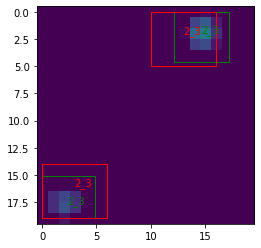
\includegraphics[width=\linewidth]{b16_8769_16616_17279_20.png}
  \endminipage\hfill
  \minipage{0.32\textwidth}
    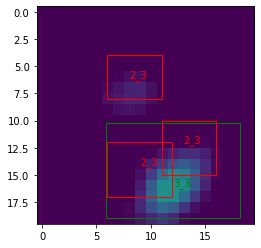
\includegraphics[width=\linewidth]{b16_14003_16486_17609_20.png}
  \endminipage\hfill
  \minipage{0.32\textwidth}
  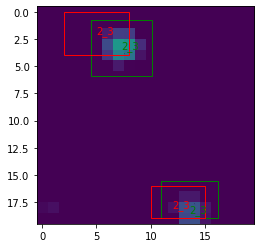
\includegraphics[width=\linewidth]{b16_14365_16926_17629_20.png}
  \endminipage\hfill
  \caption{Examples of predictions for B16 model.}
  \label{fig:b16-pred}
\end{figure}

\begin{figure}[!htb]
  \minipage{0.32\textwidth}
    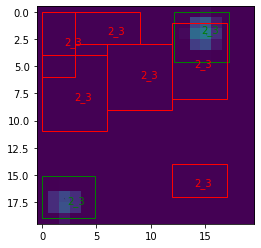
\includegraphics[width=\linewidth]{b44_8769_16616_17279_20.png}
  \endminipage\hfill
  \minipage{0.32\textwidth}
    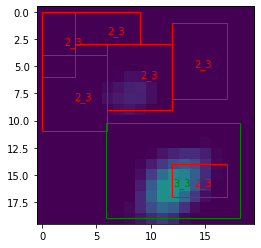
\includegraphics[width=\linewidth]{b44_14003_16486_17609_20.png}
  \endminipage\hfill
  \minipage{0.32\textwidth}
  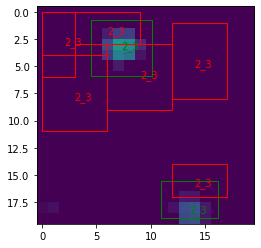
\includegraphics[width=\linewidth]{b44_14365_16926_17629_20.png}
  \endminipage\hfill
  \caption{Examples of predictions for B44 model on the same images.}
  \label{fig:b44-pred}
\end{figure}



As we can see in \ref{fig:b16-pred} a very shallow model as B16 is quite good in locating the objects: indeed, mAP score is mainly affected by the misclassification of objects of class different from "2\_3".
We will talk about this in the next chapter.

\chapter{Discussion}\label{chap:discussion}

In this work, we addressed the problem of small object detection and classification on the SKADC1 dataset by leveraging a Faster R-CNN model coded from scratch.
In particular we adopted Faster R-CNN architecture for the detection and recognition, but implemented our own backbones, for feature extraction, based on the following ideas:
\begin{itemize}
\item objects are very small, so the receptive field of the network has to be chosen accurately \cite{effective-rf};
\item objects have very simple shapes, so there is no need for a very deep convolutional pipeline;
\item objects are very similar, so there is no need for a large dataset;
\item the vast majority of objects are isomorphic, so there is no need for image flipping and rotation during training, although we adopted augmentation when balancing the dataset;
\item the overlapping of objects is very rare, so no complex shapes are created;
\item the background is approximately uniform.
\end{itemize}

As described in \ref{chap:analysis-results} the best performing model is ...
although its mAP score is not comparable to SoTA models, trained on PASCAL-VOC dataset or COCO annotation \cite{faster-rcnn}.

The principal source of error, the one that makes mAP scores to be low, is the unbalancedness of the dataset: all the baseline networks overfitted on the most common class and this makes mAP to be low also when the object is detected.

The interesting thing is that a simple model as B16 outperforms a complex one like VGG16. [CONTROLLARE QUI]

Another interesting point is that, when balancing the dataset, as in B16\_20\_100+BD experiment, the model is not anymore able to learn in the time frame of 200 epochs. We think that this is due to the strong similarity in shape and brightness between classes (at least in the 560MHz and 1000h exposure). It could be interesting to try addressing this point by using other images of the same frequencies and different exposure time as the other channels of the input image, instead of repeating 3 times the same input image. We believe this could be a valid point because we are talking about astronomical objects which could have different emission spectrum.

We didn't take for granted the fact that the best setting was freezing the first layer in each model. Indeed it could be interesting to try letting also the first B16 model layers to learn (after having transferred learning from VGG16) and see what happens. Obviously this would require a greater computational effort.

Future improvements could be using Feature Pyramid Network as in \cite{fpn} in order to produce more accurate feature maps for smaller objects, or to implement the tweaks described in \cite{frcnn-small-obj} to enhance Faster R-CNN performance specifically for small objects.

We think also that combining the different sky image provided in the challenge, as they were different channel in an RGB image, could bring more information to the network and could lead to a performance improvements.

Another hypothesis, that we would like to test with more time, is that the Faster R-CNN network is not well suited for this specific problem: we think that it would be worth to try a system where the dection is carried out through a \textbf{segmentation} approach and, as a second step, a classifier that classifies detected objects.

\printbibliography
\end{document}
